\documentclass{article}

\usepackage{fancyhdr}
\usepackage{extramarks}
\usepackage{amsmath}
\usepackage{amsthm}
\usepackage{amsfonts}
\usepackage{tikz}
\usepackage{graphicx}
\usepackage{float}
\usepackage{listings}
\usepackage{booktabs}

%\usetikzlibrary{automata,positioning}
\usetikzlibrary{shapes, arrows}

%
% Basic Document Settings
%

\topmargin=-0.45in
\evensidemargin=0in
\oddsidemargin=0in
\textwidth=6.5in
\textheight=9.0in
\headsep=0.25in

\linespread{1.1}

\pagestyle{fancy}
\lhead{\hmwkAuthorName}
\rhead{\hmwkClass\ (\hmwkClassInstructor)}
\cfoot{\thepage}

\lstset{
  caption=\lstname,
  %backgroundcolor=\color{lightgray},
  literate={\$}{{\$}}1,
  breaklines=true,
  basicstyle=\ttfamily\small
}

\DeclareMathOperator*{\argmin}{arg\,min}
\renewcommand\headrulewidth{0.4pt}
\renewcommand\footrulewidth{0.4pt}

\setlength\parindent{0pt}

\newcommand{\hmwkTitle}{Utilizing reinforcement learning techniques to play Atari's Breakout}
\newcommand{\hmwkDueDate}{07 December 2015}
\newcommand{\hmwkClass}{Reinforcement Learning}
\newcommand{\hmwkClassInstructor}{Dr. Itamar Arel}
\newcommand{\hmwkAuthorName}{Andrew Messing, Ben Brock, and Cory Walker}

%
% Title Page
%

\title{
    \vspace{2in}
    \textmd{\textbf{\hmwkTitle}}\\
    \normalsize\vspace{0.1in}\small{Due\ on\ \hmwkDueDate}\\
    \vspace{0.1in}\large{\textit{\hmwkClassInstructor}}
    \vspace{3in}
}

\author{\textbf{\hmwkAuthorName}}
\date{}

\renewcommand{\part}[1]{\textbf{\large Part \Alph{partCounter}}\stepcounter{partCounter}\\}

%
% Various Helper Commands
%

% Alias for the Solution section header
\newcommand{\solution}{ \hfill \break \break \textbf{Solution} \hfill \break \break}

\begin{document}

\maketitle

\pagebreak

\begin{abstract}
We demonstrate the performance of two different reinforcement learning methods, basic Q-learning using manual image processing and deep Q-learning using raw pixel input, on Atari's Breakout.  While deep reinforcement learning techniques may be generalizable across games and ultimately result in optimal performance, they require a large amount of computational resources and time for training.  By performing manual image processing to derive states, we show that similar performance can be achieved in less time using basic Q-learning.
\end{abstract}

\section{Introduction}
Deep Reinforment Learning is a relatively new approach to learn to control agents via high dimensional sensory inputs like vision in speech. This project compares success of a specific feature based reinforcement learning approach to a deep reinforcement learning one using the atari game breakout and the Arcade Learning Environment.

\section{Breakout and feature extraction}
\subsection{Breakout}
Breakout is a classic arcade game developed by Atari, Inc. Similar to pong the object is to use a paddle to bounce a ball; however for breakout the paddle move horizontally and is positioned at the bottom of the screen. At the top of the screen are multiple layers of bricks. Everytime the ball collides with a brick it breaks it and the player gains points. The goal of the game is to break all the bricks, score points, and not let the ball fall below the paddle as that costs the user a life. When all the lives are gone the game is over.

  \begin{center}
  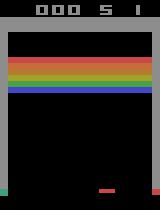
\includegraphics[width=50mm]{tmp.jpg}
  \end{center}

\subsection{Arcade Learning Environment}
The Arcade Learning Environment (ALE) is a simple object-oriented framework designed to allow researchers to test Artificial Intelligence agents to play Atari 2600 games. The agent can receive the game frames and ram and is given access to the number of lives, the score, and other information from the game. Then the agent can use this to come with an action that it would send back to the ALE. The controller that is simulated contains a joystick, an action button, and a couple of menu buttons that total to about 20 possible actions including the buttons being pressed and the joystick being moved in one of eight directions.
\\\\
For breakout specifically there are three actions that contribute to the game: move the joystick left, move the joystick right, and do nothing.

\subsection{Feature Extraction}
To extract features for the non-Deep reinforcement learning agent image processing was used to capture the paddle and the ball's position. While the paddle maintained one of two colors making it relatively easy to extract, the ball changes colors as it goes by the brick layers to the color of that brick layer and when it is in open space to the color of the paddle. 

\begin{figure}
  \caption{Feature extraction performed on a frame from Breakout.  The white dots indicate the detected x and y coordinates of the paddle and ball.}
  \begin{center}
    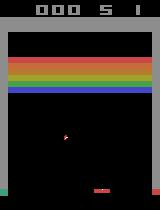
\includegraphics[scale=.75]{tmp2.jpg}
  \end{center}
\end{figure}

\section{Reinforcement learning}
\subsection{Introduction}
The Breakout problem is the problem of playing the game of Breakout while maximizing the score received.  Our RL agent controls the paddle and, at each timestep of the ALE engine, has three possible actions: to move the paddle to the left, to hold the paddle still, or to move the paddle to the left.  The optimal action will depend depend on the position of the paddle, the position of the ball, and possibly the position of the blocks overhead.  Here, we will present a simple Q-learning approach to solving the Breakout problem.  First, we will discuss the formulation of the problem as a Markov Decision Process (MDP), then the design and implementation of our Q-learning approach to training an RL agent to solve Breakout.  Then, we will discuss the training results and performance of our agent.
\subsection{Formulation as an MDP}
In our formulation of Breakout, the RL agent has three possible states, which are each derived from the relative x-coordinate position of the ball and paddle.  Either the ball is to the left of the paddle (state 1), the ball is directly on top of the paddle (state 2), or the ball is to the right of the paddle (state 3).  In our formulation, our RL agent is given a state value and the opportunity to perform an action at each timestep of the ALE.  The RL agent may perform one of three actions: the RL agent may choose to move the paddle to the left, to the right, or to hold the paddle still.  When the ball drops below the paddle (losing a game life), the RL agent will receive a reward of -10.  At all other timesteps, the RL agent will receive a reward of 0.
\\\\
We have chosen this formulation because of its simplicity.  While a truly optimal Breakout player may use the position of the bricks to inform its decisions about how to hit the ball, it is our hypothesis that a player which simply attempts to hit the ball may be very nearly optimal.  We wish to demonstrate that a very simple formulation may achieve high performance if it is well-tuned to the attributes of the system.
\subsection{Q-Learning Method}
We use Q-learning with elligibility traces to train our RL agent to solve Breakout.

\section{Deep reinforcement learning}
Cory's section goes here.
\subsection{Deep Q network}
\subsection{DQN variations}
\subsection{Double DQN formulation}
\subsection{Implementation}
\subsection{Results}
\begin{figure}[H]
  \centering
  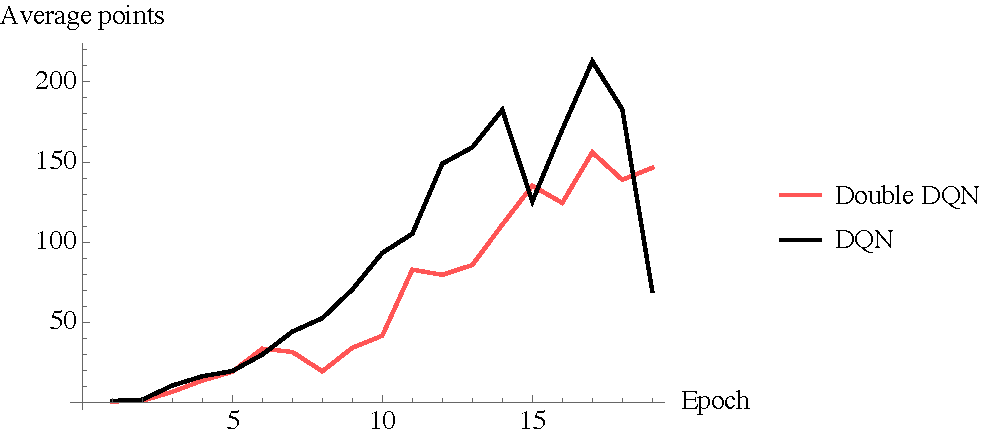
\includegraphics[width=120mm]{dqn_rewardper.pdf}
  \caption{Example figure.}
\end{figure}
Each epoch takes about an hour. Stopped after $\sim 20$ hours.\\

\section{Design challenges}
Put design challenges here.

\section{Summary}
A summary goes here.

%\section{Appendix}
%\begin{center}
  %\lstinputlisting{/Users/cwalker32/Documents/LaTeX/ece_517/proj2/et.m}
%\end{center}


\pagebreak

\end{document}
